%%%%%%%%%%%%%%%%%%%%%%%%%%%%%%%%%%%%%%%%
% Beamer Presentation
% LaTeX Template
% Version 1.0 (10/11/12)
%
% This template has been downloaded from:
% http://www.LaTeXTemplates.com
%
% License:
% CC BY-NC-SA 3.0 (http://creativecommons.org/licenses/by-nc-sa/3.0/)
%
%%%%%%%%%%%%%%%%%%%%%%%%%%%%%%%%%%%%%%%%%

%----------------------------------------------------------------------------------------
%   PACKAGES AND THEMES
%----------------------------------------------------------------------------------------

lass{beamer}

\mode<presentation> {

% The Beamer class comes with a number of default slide themes
% which change the colors and layouts of slides. Below this is a list
% of all the themes, uncomment each in turn to see what they look like.

%\usetheme{default}
%\usetheme{AnnArbor}
%\usetheme{Antibes}
%\usetheme{Bergen}
%\usetheme{Berkeley}
%\usetheme{Berlin}
%\usetheme{Boadilla}
%\usetheme{CambridgeUS}
%\usetheme{Copenhagen}
%\usetheme{Darmstadt}
%\usetheme{Dresden}
%\usetheme{Frankfurt}
%\usetheme{Goettingen}
%\usetheme{Hannover}
%\usetheme{Ilmenau}
%\usetheme{JuanLesPins}
%\usetheme{Luebeck}
\usetheme{Madrid}
%\usetheme{Malmoe}
%\usetheme{Marburg}
%\usetheme{Montpellier}
%\usetheme{PaloAlto}
%\usetheme{Pittsburgh}
%\usetheme{Rochester}
%\usetheme{Singapore}
%\usetheme{Szeged}
%\usetheme{Warsaw}


% As well as themes, the Beamer class has a number of color themes
% for any slide theme. Uncomment each of these in turn to see how it
% changes the colors of your current slide theme.

%\usecolortheme{albatross}
%\usecolortheme{beaver}
%\usecolortheme{beetle}
%\usecolortheme{crane}
%\usecolortheme{dolphin}
%\usecolortheme{dove}
%\usecolortheme{fly}
%\usecolortheme{lily}
%\usecolortheme{orchid}
%\usecolortheme{rose}
%\usecolortheme{seagull}
%\usecolortheme{seahorse}
%\usecolortheme{whale}
%\usecolortheme{wolverine}

%\setbeamertemplate{footline} % To remove the footer line in all slides uncomment this line
%\setbeamertemplate{footline}[page number] % To replace the footer line in all slides with a simple slide count uncomment this line

%\setbeamertemplate{navigation symbols}{} % To remove the navigation symbols from the bottom of all slides uncomment this line
}
\usepackage[utf8]{inputenc}
\usepackage{amsmath}
\usepackage{graphicx}
\graphicspath{ {images/} }
\usepackage[all,cmtip]{xy}
\usepackage{hyperref}
\usepackage{graphicx} % Allows including images
\usepackage{booktabs} % Allows the use of \toprule, \midrule and \bottomrule in tables

%----------------------------------------------------------------------------------------
%   TITLE PAGE
%----------------------------------------------------------------------------------------

\title{Hybrid systems: an introduction} % The short title appears at the bottom of every slide, the full title is only on the title page

\author{Billy} % Your name
\institute[UBA] % Your institution as it will appear on the bottom of every slide, may be shorthand to save space
{
Universidad de Buenos Aires\\ % Your institution for the title page
\medskip
\textit{billy.mosse@gmail.com} \\ % Your email address


\tiny{Robé el template de internet} \\

}
\date{\today} % Date, can be changed to a custom date

\begin{document}

\begin{frame}
\titlepage % Print the title page as the first slide
\end{frame}

\begin{frame}
\frametitle{Overview} % Table of contents slide, comment this block out to remove it
\tableofcontents % Throughout your presentation, if you choose to use \section{} and \subsection{} commands, these will automatically be printed on this slide as an overview of your presentation
\end{frame}

%----------------------------------------------------------------------------------------
%   PRESENTATION SLIDES
%----------------------------------------------------------------------------------------

%------------------------------------------------
\section{Introduction} % Sections can be created in order to organize your presentation into discrete blocks, all sections and subsections are automatically printed in the table of contents as an overview of the talk
%------------------------------------------------

%\subsection{Subsection Example} % A subsection can be created just before a set of slides with a common theme to further break down your presentation into chunks

%\begin{frame}
%\frametitle{Tipos de juegos que conozco}



%\end{frame}

%------------------------------------------------

\subsection{A little background}
\begin{frame}

\frametitle{Tipos de juegos que conozco: combinatoriales}

Rapid progress in hardware and software $\rightarrow$ 
ambitious projects $\rightarrow$ costly ad-hoc integration and validation of systems. \\
Slowly incremental distributed systems "sin usar todo al mango"\\
more people $\rightarrow$ we need new paradigm: we can't afford a central control, but it would be nice to have a central authority so we can take smart decisions with the information from all the system.\\
hierarchic (esto no se escribe asi) system, more or less autonomous functions, and harmony.

"Studies [citation needed] indicate that, if there is no change to the structure of ATC, then by the year 2015 there could be a major accident every 7 to 10 days."
\end{frame}
%------------------------------------------------


\begin{frame}
	\frametitle{Hierarchical structure}

	Discrete controls of the system (high level)
	%$\xrightarrow{\phantom{texttexttext}$
	INFORMATION GOES UP
	COMMANDS GO DOWN	
	
	Continuous control laws of the world (low level)
\end{frame}


\begin{frame}
	\frametitle{Problems we could resolve}
\begin{itemize}
	\item Automated highway systems
	\item Air traffic control
	\item Groups of anmanned aerial vehicles
	\item Underwater autonomous vehicles
	\item Mobile offshore platforms

\end{itemize}
\end{frame}


\begin{frame}
	\frametitle{Literature on hybrid systems}
	 1) Idea: extend techniques for finite state automata to include systems with simple continuous dynamics.
	 
	 How? Model checking and/or deductive theorem proving
	 Emphasis: computability, decidability. "Does the problem satisfy the specification" is decidable?
	 
	Models and decidability
results have been obtained for timed automata [4], linear hybrid automata [3], and hybrid
input/output automata [59]. 

Decidability results for linear hybrid automata are
fairly narrow.  For all but the simplest continuous linear dynamics (two-dimensional rect-
angular differential inclusions), reachability properties are semi-decidable at best, and in
most cases undecidable	 
	 
	 See https://www.irif.fr/~asarin/papers/incl.pd, Section 2
\end{frame}


\begin{frame}

Un/decidability sometimes may be proven by (bi)simulation

\begin{itemize}
	\item Dynamical systems: topological equivalence and homomorphism
	\item Hybrid systems:
		\begin{itemize}
			\item Not easy
			\item Ad hoc definition that must include reachability: if system A simulates system B then it provides a reduction from reachability problem for A to the one for B
		\end{itemize}
\end{itemize}

In the end, it's another reduction to Halt. 
(See http://www.sciencedirect.com/science/article/pii/030439759400228B
. Also, http://www.sciencedirect.com/science/article/pii/S0890540112000028)
Interestingly, it uses some tools from Topology and Geometry.)\end{frame}


\begin{frame}
	\frametitle{Literature on hybrid systems}
	 2) Idea:  extend the standard modeling, reachability and stability
analyses, and controller design techniques in continuous state space and continuous time dynamical systems and control to capture the interaction between the continuous
and discrete dynamics.

%TODO remove/add references from pdf here

Tools extended:  stability theory [17], optimal control [17, 53, 67], and control of
discrete event systems [49, 38]

ne area in which results have been hard
to come by is the efficient
computation
of reachable sets for hybrid systems whose dynamics
are nonlinear or are of order greater than one.  Only recently [<2007], some attempts to directly
approach this problem have been reported in the literature 
\end{frame}

\begin{frame}
	Stability theory addresses the stability of solutions of differential equations and of trajectories of dynamical systems under small perturbations of initial conditions.
\end{frame}

\begin{frame}
	\frametitle{Optimal control}
	x $\leftarrow$ state
	u $\leftarrow$ controllable parameters
		
	
	minimize 	$J = \psi[x(T)] + \int_{0}^{T} \ell(u,x(t)) dt$
\end{frame}

\begin{frame}
	One solution:
	1) discretization of the problem
	2) Principle of Optimality: An optimal policy has the property that whatever the initial state and initial decision are, the remaining decisions must constitute an optimal policy with regard to the state resulting from the first decision. (See Bellman, 1957, Chap. III.3.)
	3) Go backwards.
	Problems: costly; "curse of dimensionality"
\end{frame}

\begin{frame}
	Another solution: gradient descent?
\end{frame}

\begin{frame}
	Another solution: perturbate ($u$) + differentiate, and get 4 necessary conditions (stated in
%TODO add link
 %https://en.wikipedia.org/wiki/Pontryagin%27s_maximum_principle
	
%TODO add link
	See %http://www.bauer.uh.edu/rsusmel/phd/MR-15.pdf for some nice examples.
	(Or let's do together the "a minimizing curve in the plane is a straight line) % - 1 + f'^2
	% Remember the fundamental lemma of calculus of variations
\end{frame}




\begin{frame}
\frametitle{What's interesting}
\begin{itemize}
	\item Continuity with respect to initial conditions (for simulations)
	\begin{itemize}
		\item Using topology (homotopy theory) tools (Sokorod topology for paths) - not practical (See %https://www.researchgate.net/publication/3792882_Regularity_of_solutions_and_homotopic_equivalence_for_hybrid_systems)
		\item %https://www.researchgate.net/profile/Karl_Johansson2/publication/2920336_Dynamical_Properties_of_Hybrid_Automata/links/02e7e51aa0db91ccdc000000.pdf
		is a more practical (and concrete?) but still limited method
	\item 
	\end{itemize}
	\item Well-posedness (existence and uniqueness of solutions)
\end{itemize}


\end{frame}

%------------------------------------------------


%------------------------------------------------
\subsection{Problems}

\begin{frame}
\frametitle{Zeno executions}

An execution is called Zeno, if it contains an infinite number of transitions in a finite
amount of time. An automaton is called Zeno if it accepts a Zeno execution.

Example: bouncing ball

Problems: 
\begin{itemize}
	\item Semantical: how it is defined beyond the Zeno time?
	\item Analysis: induction and reachability proofs become suspect
	\item Controller synthesis: it can cheat by forcing time to converge
	\item Simulation: it stalls at Zeno time
\end{itemize}

\end{frame}

%------------------------------------------------



%------------------------------------------------


\begin{frame}
	\frametitle{Resolving the Zeno phenomenon}
	The only known conditions to characterize the Zeno phenomenon are fairly trivial.
	
	A regularization approach (of the automata), inspired by the method used in differential equations.
	
	E.g. 
	\begin{itemize}
		\item	ater tank automaton: the switch takes $\epsilon$ to activate.
		\item Bouncing ball: each bounce takes $\epsilon$ (meanwhile, gravity still applies) 		
	\end{itemize}
	
	As $\varepsilon \rightarrow 0$, then the non-Zeno automata $H_\varepsilon $ converges to the original Zeno automata ($\phi_\varepsilon : Q_\varepsilon \times X_\varepsilon \rightarrow Q \times X$ converges in the Skorohod metric)
	
	 See %http://users.ece.gatech.edu/magnus/Papers/ZenoAutomata.pdf
			
\end{frame}

\subsection{Some definitions}

\begin{frame}
	\frametitle{Some basic descriptions: Timed automata}
	See 
%TODO	
	%www.cis.upenn.edu/~alur/TCS94.pdf and https://en.wikipedia.org/wiki/Timed_automaton
	
	Timed automata:
	\begin{itemize}
		\item Nice augmentation of $\omega$-automata (Seen in class)
		\item Words are timed (each letter is presented at a certain time)
		\item Time satisfies monotonicity and progress
		\item Clocks that can be reseted (in the automata, not...the language)
		\item Reachability and eventuality properties are decidable
	\end{itemize}
\end{frame}

\begin{frame}
	\frametitle{Some basic descriptions: other automatas}
	
	\begin{itemize}
		\item Linear hybrid automata: models $A\dot{x}\leq b$. Decidability results are fairly narrow. TODO: research how do they model discrete actions.
		\item Hybrid input/output automata. See
		%TODO %http://citeseerx.ist.psu.edu/viewdoc/download?doi=10.1.1.13.1457&rep=rep1&type=pdf and perhaps http://www.ita.cs.ru.nl/publications/papers/fvaan/hioaslides.pdf
	Permits:
	\begin{itemize}
		\item Easy decomposition of description and analysis
		\item Showing that one automata implements another one
		\item Showing that there isn't Zeno behaviour under 
	\end{itemize}
		
	\end{itemize}
\end{frame}



\begin{frame}
\frametitle{The language}
	The modelling language must be
\begin{itemize}
	\item descriptive: to model how discrete evolution affects and is affected by continuous evolution, to allow non-deterministic models to capture uncertainty
	\item composable
	\item abstractable, to refine problems down and compose results up
\end{itemize}

\end{frame}

\begin{frame}
	\frametitle{One of the languages: Hybrid Automata}
	$H = (Q, X, Init, f, Inv/Dom, E, G, R)$ %Inv y Dom son intercambiables en el libro
	
	\begin{itemize}
		\item $Q$ (countable) is a set of discrete variables
		\item $X$ is a set of continuous variables
		\item $Init \subset Q \times X$ is a set of initial states
		\item $f: Q \times X \rightarrow TX$ is a vector field: it usually describes the derivative of the continuous variable
		\item $Inv/Dom: Q \rightarrow P(X)$ assigns to each $q \in Q$ an invariant set
		\item $E \subset Q \times Q$ is a collection of discrete transitions
		\item $G : E \rightarrow P(X)$ assigns to each $e=(q,q') \in E$ a guard.
		\item $R : E \times X \rightarrow P(X)$ assigns to each $e = (q,q') \in E$ and $x \in X$ a reset relation
	\end{itemize}
	
Example: Water Tank System. Two tanks are leaking are at constant rates ($v_1,v_2$) respectively. Water is added constantly though a hose controlled by an instantaneous switch.

¿Can the water of both tanks ($x_1,x_2$) be kept above ($r_1,r_2$)?
\end{frame}

\begin{frame}
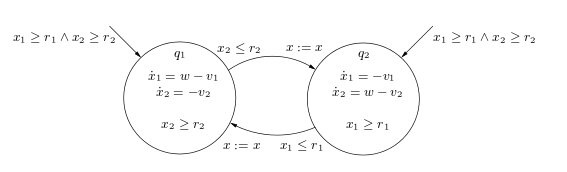
\includegraphics[scale=1]{tank_system.png}
\end{frame}

\begin{frame}
	\frametitle{Definition: Hybrid time set.}
	
	A hybrid time set is a set $\tau = \{I_0,\cdots,I_N\}$ (finite or infinite) of almost-disjoint ordered intervals.
	\begin{itemize}
		\item $I_i = [\tau_i, \tau'_i]$ with $\tau'_i = \tau_{i+1}\ \forall\ i < N$
		\item If $N < \infty$ then $I_N$ might be $[\tau_N, \tau'_N)$
	\end{itemize}	 
	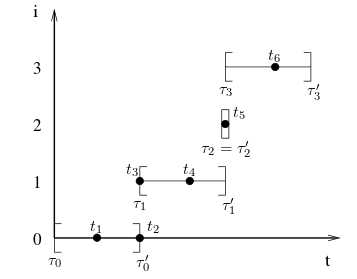
\includegraphics[scale=0.7]{partition.png}
\end{frame}

\begin{frame}
	\frametitle{Definition: execution}
	
	Definition: A hybrid trajectory is a triple ($\tau,q,x$), with the hybrid time set $\tau = \{I_i\}$, and two sequences of functions $q = \{q_i\}, x = \{x_i\}$, with $q_i(.),x_i(.) : I_i \rightarrow \mathbb{R}^n$
	
	Definition: an execution$\mathbb{H}$ of a hybrid automaton $H$ is a hybrid trajectory ($\tau,q,x$) satisfying:
	\begin{itemize}
		\item Initial condition: $q(0),x(0) \in Init$
		\item Discrete evolution: the discrete transitions must be valid and the guards must be satisfied
		\item Continuous evolution: the continuous variables must be reseted after each transition, and between them they must belong to the domain, $q_i$ must be constant over $I_i$
	\end{itemize}
\end{frame}

\begin{frame}
	\frametitle{Controllers: a really brief introduction}
	
	\begin{itemize}
		\item We add input variables $v \in V$ (continuous/discrete and controls(U)/disturbances (D))
		%(T \times Q \times X)^*
		\item $C : \mathbb{H} \rightarrow 2^U$ a controller that restricts the control input variables allowed at the final state
		\item $\mathbb{H}_C$ the set of "closed loop causal executions" (executions with inputs always approved by $C$)
		\item $C$ satisfies ($Q \cap X, \square F$) if $\square F(\chi) = True\ \forall\ \chi \in \mathbb{H}$. Problems: Zeno, blocked executions		
	\end{itemize}
\end{frame}

\begin{frame}
	Proposition 6.2 %TODO https://pdfs.semanticscholar.org/6c3c/c35e9e723a586390244565cfa0081cc86f7e.pdf
	
	A controller satisfying	 ($Q \cap X, \square F$) exists if and only if a memorless controller satisfying ($Q \cap X, \square F$) exists.

Idea of the proof: a drawing. Also, we must strongly use that valid executions and properties are "locally memoryless"

(By contradiction)

1. Assume $\chi_1,\chi_2$, reaching $(x,q)$ with $C(\chi_1) \neq C(\chi_2)$.
2. Then, append $\chi'$ to $\chi_2$, but with a control rule applied to $\chi_2 \chi'$ so that $F$ doesn't hold somewhere. (We can assume we can do it, because we are supposing a memoryless strategy doesn't exist)
3. $\chi_2 \chi'$ breaks down at some time $t$. $\chi_1 \chi'$ is a valid executions as executions are memoryless, and also breaks down at time $t$. Absurd! Because $\chi_1 \chi'$ was also validated by the controller, by construction, and the controller satisfied ($Q \cap X, \square F$)

\end{frame}




\section{Bibliografía}

\begin{frame}
\frametitle{Bibliografía}

\href{<http://www.math.ucla.edu/~tom/Game_Theory/comb.pdf>}{Game Theory, Ferguson}

\end{frame}


%
%\begin{frame}
%\frametitle{Multiple Columns}
%\begin{columns}[c] % The "c" option specifies centered vertical alignment while the "t" option is used for top vertical alignment
%
%\column{.45\textwidth} % Left column and width
%\textbf{Heading}
%\begin{enumerate}
%\item Statement
%\item Explanation
%\item Example
%\end{enumerate}
%
%\column{.5\textwidth} % Right column and width
%Lorem ipsum dolor sit amet, consectetur adipiscing elit. Integer lectus nisl, ultricies in feugiat rutrum, porttitor sit amet augue. Aliquam ut tortor mauris. Sed volutpat ante purus, quis accumsan dolor.
%
%\end{columns}
%\end{frame}
%
%
%
%%------------------------------------------------
%\section{Second Section}
%%------------------------------------------------
%
%\begin{frame}
%\frametitle{Table}
%\begin{table}
%\begin{tabular}{l l l}
%\toprule
%\textbf{Treatments} & \textbf{Response 1} & \textbf{Response 2}\\
%\midrule
%Treatment 1 & 0.0003262 & 0.562 \\
%Treatment 2 & 0.0015681 & 0.910 \\
%Treatment 3 & 0.0009271 & 0.296 \\
%\bottomrule
%\end{tabular}
%\caption{Table caption}
%\end{table}
%\end{frame}
%
%%------------------------------------------------
%
%\begin{frame}
%\frametitle{Theorem}
%\begin{theorem}[Mass--energy equivalence]
%$E = mc^2$
%\end{theorem}
%\end{frame}
%
%%------------------------------------------------
%
%\begin{frame}[fragile] % Need to use the fragile option when verbatim is used in the slide
%\frametitle{Verbatim}
%\begin{example}[Theorem Slide Code]
%\begin{verbatim}
%\begin{frame}
%\frametitle{Theorem}
%\begin{theorem}[Mass--energy equivalence]
%$E = mc^2$
%\end{theorem}
%\end{frame}\end{verbatim}
%\end{example}
%\end{frame}
%
%%------------------------------------------------
%
%\begin{frame}
%\frametitle{Figure}
%Uncomment the code on this slide to include your own image from the same directory as the template .TeX file.
%%\begin{figure}
%%\includegraphics[width=0.8\linewidth]{test}
%%\end{figure}
%\end{frame}
%
%%------------------------------------------------
%
%\begin{frame}[fragile] % Need to use the fragile option when verbatim is used in the slide
%\frametitle{Citation}
%An example of the \verb|\cite| command to cite within the presentation:\\~
%
%This statement requires citation \cite{p1}.
%\end{frame}
%
%%------------------------------------------------
%
%\begin{frame}
%\frametitle{References}
%\footnotesize{
%\begin{thebibliography}{99} % Beamer does not support BibTeX so references must be inserted manually as below
%\bibitem[Smith, 2012]{p1} John Smith (2012)
%\newblock Title of the publication
%\newblock \emph{Journal Name} 12(3), 45 -- 678.
%\end{thebibliography}
%}
%\end{frame}
%
%%------------------------------------------------
%
%\begin{frame}
%\Huge{\centerline{The End}}
%\end{frame}
%
%%----------------------------------------------------------------------------------------

\end{document}	